% Created by tikzDevice version 0.12.6 on 2025-08-19 18:36:12
% !TEX encoding = UTF-8 Unicode
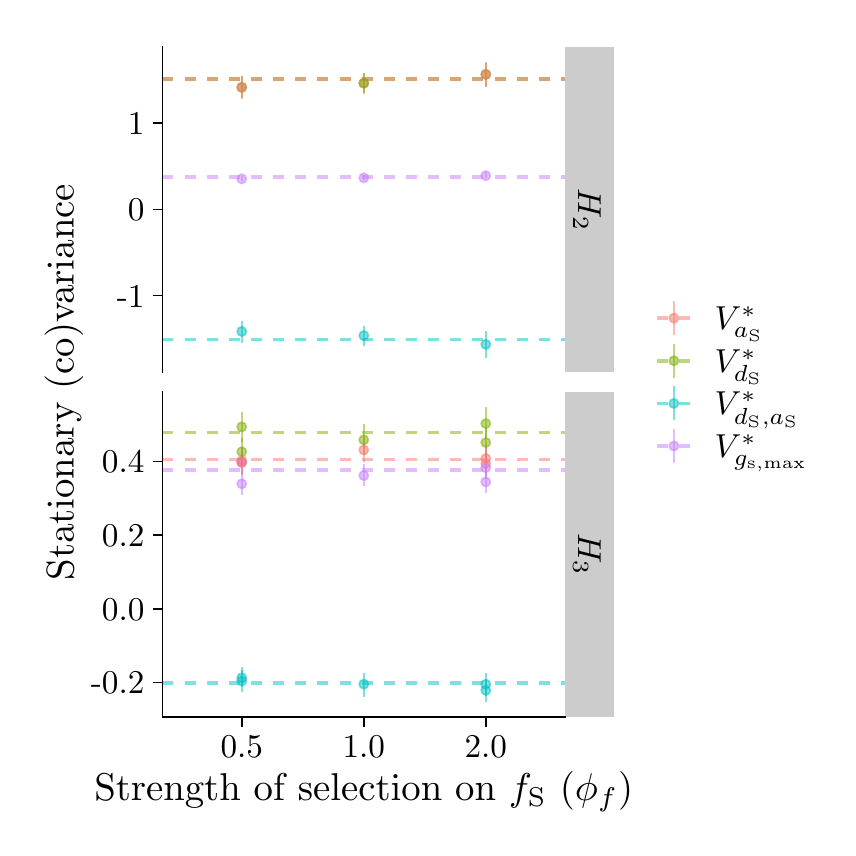
\begin{tikzpicture}[x=1pt,y=1pt]
\definecolor{fillColor}{RGB}{255,255,255}
\path[use as bounding box,fill=fillColor,fill opacity=0.00] (0,0) rectangle (289.08,289.08);
\begin{scope}
\path[clip] ( 48.69,164.52) rectangle (194.20,282.08);
\definecolor{drawColor}{RGB}{124,174,0}

\path[draw=drawColor,draw opacity=0.50,line width= 1.3pt,dash pattern=on 4pt off 4pt ,line join=round] ( 48.69,270.45) -- (194.20,270.45);
\definecolor{drawColor}{RGB}{248,118,109}

\path[draw=drawColor,draw opacity=0.50,line width= 1.3pt,dash pattern=on 4pt off 4pt ,line join=round] ( 48.69,270.45) -- (194.20,270.45);
\definecolor{drawColor}{RGB}{0,191,196}

\path[draw=drawColor,draw opacity=0.50,line width= 1.3pt,dash pattern=on 4pt off 4pt ,line join=round] ( 48.69,176.37) -- (194.20,176.37);
\definecolor{drawColor}{RGB}{199,124,255}

\path[draw=drawColor,draw opacity=0.50,line width= 1.3pt,dash pattern=on 4pt off 4pt ,line join=round] ( 48.69,235.17) -- (194.20,235.17);
\definecolor{drawColor}{RGB}{0,191,196}

\path[draw=drawColor,draw opacity=0.50,line width= 0.7pt,line join=round] (165.54,169.86) -- (165.54,179.30);
\definecolor{drawColor}{RGB}{124,174,0}

\path[draw=drawColor,draw opacity=0.50,line width= 0.7pt,line join=round] (165.54,267.59) -- (165.54,276.74);
\definecolor{drawColor}{RGB}{248,118,109}

\path[draw=drawColor,draw opacity=0.50,line width= 0.7pt,line join=round] (165.54,267.47) -- (165.54,276.48);
\definecolor{drawColor}{RGB}{124,174,0}

\path[draw=drawColor,draw opacity=0.50,line width= 0.7pt,line join=round] ( 77.35,263.50) -- ( 77.35,271.70);
\definecolor{drawColor}{RGB}{248,118,109}

\path[draw=drawColor,draw opacity=0.50,line width= 0.7pt,line join=round] ( 77.35,263.43) -- ( 77.35,271.46);
\definecolor{drawColor}{RGB}{0,191,196}

\path[draw=drawColor,draw opacity=0.50,line width= 0.7pt,line join=round] ( 77.35,175.23) -- ( 77.35,182.92);
\definecolor{drawColor}{RGB}{248,118,109}

\path[draw=drawColor,draw opacity=0.50,line width= 0.7pt,line join=round] (121.45,265.15) -- (121.45,272.68);
\definecolor{drawColor}{RGB}{0,191,196}

\path[draw=drawColor,draw opacity=0.50,line width= 0.7pt,line join=round] (121.45,174.00) -- (121.45,181.40);
\definecolor{drawColor}{RGB}{124,174,0}

\path[draw=drawColor,draw opacity=0.50,line width= 0.7pt,line join=round] (121.45,265.38) -- (121.45,272.59);
\definecolor{drawColor}{RGB}{199,124,255}

\path[draw=drawColor,draw opacity=0.50,line width= 0.7pt,line join=round] (165.54,234.62) -- (165.54,236.79);

\path[draw=drawColor,draw opacity=0.50,line width= 0.7pt,line join=round] ( 77.35,233.53) -- ( 77.35,235.45);

\path[draw=drawColor,draw opacity=0.50,line width= 0.7pt,line join=round] (121.45,233.91) -- (121.45,235.78);
\definecolor{drawColor}{RGB}{0,191,196}
\definecolor{fillColor}{RGB}{0,191,196}

\path[draw=drawColor,draw opacity=0.50,line width= 0.6pt,line join=round,line cap=round,fill=fillColor,fill opacity=0.50] (165.54,174.63) circle (  1.69);
\definecolor{drawColor}{RGB}{124,174,0}
\definecolor{fillColor}{RGB}{124,174,0}

\path[draw=drawColor,draw opacity=0.50,line width= 0.6pt,line join=round,line cap=round,fill=fillColor,fill opacity=0.50] (165.54,272.21) circle (  1.69);
\definecolor{drawColor}{RGB}{248,118,109}
\definecolor{fillColor}{RGB}{248,118,109}

\path[draw=drawColor,draw opacity=0.50,line width= 0.6pt,line join=round,line cap=round,fill=fillColor,fill opacity=0.50] (165.54,272.18) circle (  1.69);
\definecolor{drawColor}{RGB}{124,174,0}
\definecolor{fillColor}{RGB}{124,174,0}

\path[draw=drawColor,draw opacity=0.50,line width= 0.6pt,line join=round,line cap=round,fill=fillColor,fill opacity=0.50] ( 77.35,267.53) circle (  1.69);
\definecolor{drawColor}{RGB}{248,118,109}
\definecolor{fillColor}{RGB}{248,118,109}

\path[draw=drawColor,draw opacity=0.50,line width= 0.6pt,line join=round,line cap=round,fill=fillColor,fill opacity=0.50] ( 77.35,267.51) circle (  1.69);
\definecolor{drawColor}{RGB}{0,191,196}
\definecolor{fillColor}{RGB}{0,191,196}

\path[draw=drawColor,draw opacity=0.50,line width= 0.6pt,line join=round,line cap=round,fill=fillColor,fill opacity=0.50] ( 77.35,179.31) circle (  1.69);
\definecolor{drawColor}{RGB}{248,118,109}
\definecolor{fillColor}{RGB}{248,118,109}

\path[draw=drawColor,draw opacity=0.50,line width= 0.6pt,line join=round,line cap=round,fill=fillColor,fill opacity=0.50] (121.45,269.02) circle (  1.69);
\definecolor{drawColor}{RGB}{0,191,196}
\definecolor{fillColor}{RGB}{0,191,196}

\path[draw=drawColor,draw opacity=0.50,line width= 0.6pt,line join=round,line cap=round,fill=fillColor,fill opacity=0.50] (121.45,177.81) circle (  1.69);
\definecolor{drawColor}{RGB}{124,174,0}
\definecolor{fillColor}{RGB}{124,174,0}

\path[draw=drawColor,draw opacity=0.50,line width= 0.6pt,line join=round,line cap=round,fill=fillColor,fill opacity=0.50] (121.45,269.01) circle (  1.69);
\definecolor{drawColor}{RGB}{199,124,255}
\definecolor{fillColor}{RGB}{199,124,255}

\path[draw=drawColor,draw opacity=0.50,line width= 0.6pt,line join=round,line cap=round,fill=fillColor,fill opacity=0.50] (165.54,235.62) circle (  1.69);

\path[draw=drawColor,draw opacity=0.50,line width= 0.6pt,line join=round,line cap=round,fill=fillColor,fill opacity=0.50] ( 77.35,234.45) circle (  1.69);

\path[draw=drawColor,draw opacity=0.50,line width= 0.6pt,line join=round,line cap=round,fill=fillColor,fill opacity=0.50] (121.45,234.81) circle (  1.69);
\end{scope}
\begin{scope}
\path[clip] ( 48.69, 39.96) rectangle (194.20,157.52);
\definecolor{drawColor}{RGB}{124,174,0}

\path[draw=drawColor,draw opacity=0.50,line width= 1.3pt,dash pattern=on 4pt off 4pt ,line join=round] ( 48.69,142.78) -- (194.20,142.78);
\definecolor{drawColor}{RGB}{248,118,109}

\path[draw=drawColor,draw opacity=0.50,line width= 1.3pt,dash pattern=on 4pt off 4pt ,line join=round] ( 48.69,132.98) -- (194.20,132.98);
\definecolor{drawColor}{RGB}{0,191,196}

\path[draw=drawColor,draw opacity=0.50,line width= 1.3pt,dash pattern=on 4pt off 4pt ,line join=round] ( 48.69, 52.19) -- (194.20, 52.19);
\definecolor{drawColor}{RGB}{199,124,255}

\path[draw=drawColor,draw opacity=0.50,line width= 1.3pt,dash pattern=on 4pt off 4pt ,line join=round] ( 48.69,129.32) -- (194.20,129.32);
\definecolor{drawColor}{RGB}{124,174,0}

\path[draw=drawColor,draw opacity=0.50,line width= 0.7pt,line join=round] (165.54,140.53) -- (165.54,152.18);

\path[draw=drawColor,draw opacity=0.50,line width= 0.7pt,line join=round] (121.45,134.79) -- (121.45,145.72);

\path[draw=drawColor,draw opacity=0.50,line width= 0.7pt,line join=round] ( 77.35,139.22) -- ( 77.35,150.03);

\path[draw=drawColor,draw opacity=0.50,line width= 0.7pt,line join=round] (165.54,134.06) -- (165.54,144.28);
\definecolor{drawColor}{RGB}{248,118,109}

\path[draw=drawColor,draw opacity=0.50,line width= 0.7pt,line join=round] (165.54,128.56) -- (165.54,138.69);

\path[draw=drawColor,draw opacity=0.50,line width= 0.7pt,line join=round] ( 77.35,127.70) -- ( 77.35,137.71);
\definecolor{drawColor}{RGB}{124,174,0}

\path[draw=drawColor,draw opacity=0.50,line width= 0.7pt,line join=round] ( 77.35,130.86) -- ( 77.35,140.82);
\definecolor{drawColor}{RGB}{248,118,109}

\path[draw=drawColor,draw opacity=0.50,line width= 0.7pt,line join=round] (165.54,127.04) -- (165.54,136.74);

\path[draw=drawColor,draw opacity=0.50,line width= 0.7pt,line join=round] (121.45,132.07) -- (121.45,141.07);
\definecolor{drawColor}{RGB}{199,124,255}

\path[draw=drawColor,draw opacity=0.50,line width= 0.7pt,line join=round] ( 77.35,127.79) -- ( 77.35,136.57);
\definecolor{drawColor}{RGB}{248,118,109}

\path[draw=drawColor,draw opacity=0.50,line width= 0.7pt,line join=round] ( 77.35,127.54) -- ( 77.35,136.20);
\definecolor{drawColor}{RGB}{0,191,196}

\path[draw=drawColor,draw opacity=0.50,line width= 0.7pt,line join=round] (121.45, 47.23) -- (121.45, 55.86);

\path[draw=drawColor,draw opacity=0.50,line width= 0.7pt,line join=round] (165.54, 45.30) -- (165.54, 53.79);
\definecolor{drawColor}{RGB}{199,124,255}

\path[draw=drawColor,draw opacity=0.50,line width= 0.7pt,line join=round] (165.54,126.07) -- (165.54,134.38);

\path[draw=drawColor,draw opacity=0.50,line width= 0.7pt,line join=round] (121.45,123.38) -- (121.45,131.58);

\path[draw=drawColor,draw opacity=0.50,line width= 0.7pt,line join=round] ( 77.35,120.23) -- ( 77.35,128.37);

\path[draw=drawColor,draw opacity=0.50,line width= 0.7pt,line join=round] (165.54,120.78) -- (165.54,128.84);
\definecolor{drawColor}{RGB}{0,191,196}

\path[draw=drawColor,draw opacity=0.50,line width= 0.7pt,line join=round] (165.54, 47.73) -- (165.54, 55.72);

\path[draw=drawColor,draw opacity=0.50,line width= 0.7pt,line join=round] ( 77.35, 49.12) -- ( 77.35, 57.09);

\path[draw=drawColor,draw opacity=0.50,line width= 0.7pt,line join=round] ( 77.35, 50.84) -- ( 77.35, 57.90);
\definecolor{drawColor}{RGB}{124,174,0}
\definecolor{fillColor}{RGB}{124,174,0}

\path[draw=drawColor,draw opacity=0.50,line width= 0.6pt,line join=round,line cap=round,fill=fillColor,fill opacity=0.50] (165.54,146.02) circle (  1.69);

\path[draw=drawColor,draw opacity=0.50,line width= 0.6pt,line join=round,line cap=round,fill=fillColor,fill opacity=0.50] (121.45,140.14) circle (  1.69);

\path[draw=drawColor,draw opacity=0.50,line width= 0.6pt,line join=round,line cap=round,fill=fillColor,fill opacity=0.50] ( 77.35,144.83) circle (  1.69);

\path[draw=drawColor,draw opacity=0.50,line width= 0.6pt,line join=round,line cap=round,fill=fillColor,fill opacity=0.50] (165.54,139.16) circle (  1.69);
\definecolor{drawColor}{RGB}{248,118,109}
\definecolor{fillColor}{RGB}{248,118,109}

\path[draw=drawColor,draw opacity=0.50,line width= 0.6pt,line join=round,line cap=round,fill=fillColor,fill opacity=0.50] (165.54,133.40) circle (  1.69);

\path[draw=drawColor,draw opacity=0.50,line width= 0.6pt,line join=round,line cap=round,fill=fillColor,fill opacity=0.50] ( 77.35,132.59) circle (  1.69);
\definecolor{drawColor}{RGB}{124,174,0}
\definecolor{fillColor}{RGB}{124,174,0}

\path[draw=drawColor,draw opacity=0.50,line width= 0.6pt,line join=round,line cap=round,fill=fillColor,fill opacity=0.50] ( 77.35,135.84) circle (  1.69);
\definecolor{drawColor}{RGB}{248,118,109}
\definecolor{fillColor}{RGB}{248,118,109}

\path[draw=drawColor,draw opacity=0.50,line width= 0.6pt,line join=round,line cap=round,fill=fillColor,fill opacity=0.50] (165.54,131.58) circle (  1.69);

\path[draw=drawColor,draw opacity=0.50,line width= 0.6pt,line join=round,line cap=round,fill=fillColor,fill opacity=0.50] (121.45,136.48) circle (  1.69);
\definecolor{drawColor}{RGB}{199,124,255}
\definecolor{fillColor}{RGB}{199,124,255}

\path[draw=drawColor,draw opacity=0.50,line width= 0.6pt,line join=round,line cap=round,fill=fillColor,fill opacity=0.50] ( 77.35,131.93) circle (  1.69);
\definecolor{drawColor}{RGB}{248,118,109}
\definecolor{fillColor}{RGB}{248,118,109}

\path[draw=drawColor,draw opacity=0.50,line width= 0.6pt,line join=round,line cap=round,fill=fillColor,fill opacity=0.50] ( 77.35,132.05) circle (  1.69);
\definecolor{drawColor}{RGB}{0,191,196}
\definecolor{fillColor}{RGB}{0,191,196}

\path[draw=drawColor,draw opacity=0.50,line width= 0.6pt,line join=round,line cap=round,fill=fillColor,fill opacity=0.50] (121.45, 51.88) circle (  1.69);

\path[draw=drawColor,draw opacity=0.50,line width= 0.6pt,line join=round,line cap=round,fill=fillColor,fill opacity=0.50] (165.54, 49.63) circle (  1.69);
\definecolor{drawColor}{RGB}{199,124,255}
\definecolor{fillColor}{RGB}{199,124,255}

\path[draw=drawColor,draw opacity=0.50,line width= 0.6pt,line join=round,line cap=round,fill=fillColor,fill opacity=0.50] (165.54,130.11) circle (  1.69);

\path[draw=drawColor,draw opacity=0.50,line width= 0.6pt,line join=round,line cap=round,fill=fillColor,fill opacity=0.50] (121.45,127.24) circle (  1.69);

\path[draw=drawColor,draw opacity=0.50,line width= 0.6pt,line join=round,line cap=round,fill=fillColor,fill opacity=0.50] ( 77.35,124.25) circle (  1.69);

\path[draw=drawColor,draw opacity=0.50,line width= 0.6pt,line join=round,line cap=round,fill=fillColor,fill opacity=0.50] (165.54,124.96) circle (  1.69);
\definecolor{drawColor}{RGB}{0,191,196}
\definecolor{fillColor}{RGB}{0,191,196}

\path[draw=drawColor,draw opacity=0.50,line width= 0.6pt,line join=round,line cap=round,fill=fillColor,fill opacity=0.50] (165.54, 51.81) circle (  1.69);

\path[draw=drawColor,draw opacity=0.50,line width= 0.6pt,line join=round,line cap=round,fill=fillColor,fill opacity=0.50] ( 77.35, 53.00) circle (  1.69);

\path[draw=drawColor,draw opacity=0.50,line width= 0.6pt,line join=round,line cap=round,fill=fillColor,fill opacity=0.50] ( 77.35, 54.16) circle (  1.69);
\end{scope}
\begin{scope}
\path[clip] (194.20,164.52) rectangle (211.80,282.08);
\definecolor{fillColor}{gray}{0.80}

\path[fill=fillColor] (194.20,164.52) rectangle (211.80,282.08);
\definecolor{drawColor}{RGB}{0,0,0}

\node[text=drawColor,rotate=-90.00,anchor=base,inner sep=0pt, outer sep=0pt, scale=  1.20] at (198.87,223.30) {$H_2$};
\end{scope}
\begin{scope}
\path[clip] (194.20, 39.96) rectangle (211.80,157.52);
\definecolor{fillColor}{gray}{0.80}

\path[fill=fillColor] (194.20, 39.96) rectangle (211.80,157.52);
\definecolor{drawColor}{RGB}{0,0,0}

\node[text=drawColor,rotate=-90.00,anchor=base,inner sep=0pt, outer sep=0pt, scale=  1.20] at (198.87, 98.74) {$H_3$};
\end{scope}
\begin{scope}
\path[clip] (  0.00,  0.00) rectangle (289.08,289.08);
\definecolor{drawColor}{RGB}{0,0,0}

\path[draw=drawColor,line width= 0.6pt,line join=round,line cap=rect] ( 48.69, 39.96) --
	(194.20, 39.96);
\end{scope}
\begin{scope}
\path[clip] (  0.00,  0.00) rectangle (289.08,289.08);
\definecolor{drawColor}{RGB}{0,0,0}

\path[draw=drawColor,line width= 0.6pt,line join=round] ( 77.35, 36.46) --
	( 77.35, 39.96);

\path[draw=drawColor,line width= 0.6pt,line join=round] (121.45, 36.46) --
	(121.45, 39.96);

\path[draw=drawColor,line width= 0.6pt,line join=round] (165.54, 36.46) --
	(165.54, 39.96);
\end{scope}
\begin{scope}
\path[clip] (  0.00,  0.00) rectangle (289.08,289.08);
\definecolor{drawColor}{RGB}{0,0,0}

\node[text=drawColor,anchor=base,inner sep=0pt, outer sep=0pt, scale=  1.20] at ( 77.35, 25.20) {0.5};

\node[text=drawColor,anchor=base,inner sep=0pt, outer sep=0pt, scale=  1.20] at (121.45, 25.20) {1.0};

\node[text=drawColor,anchor=base,inner sep=0pt, outer sep=0pt, scale=  1.20] at (165.54, 25.20) {2.0};
\end{scope}
\begin{scope}
\path[clip] (  0.00,  0.00) rectangle (289.08,289.08);
\definecolor{drawColor}{RGB}{0,0,0}

\path[draw=drawColor,line width= 0.6pt,line join=round,line cap=rect] ( 48.69,164.52) --
	( 48.69,282.08);
\end{scope}
\begin{scope}
\path[clip] (  0.00,  0.00) rectangle (289.08,289.08);
\definecolor{drawColor}{RGB}{0,0,0}

\node[text=drawColor,anchor=base east,inner sep=0pt, outer sep=0pt, scale=  1.20] at ( 42.19,188.11) {-1};

\node[text=drawColor,anchor=base east,inner sep=0pt, outer sep=0pt, scale=  1.20] at ( 42.19,219.28) {0};

\node[text=drawColor,anchor=base east,inner sep=0pt, outer sep=0pt, scale=  1.20] at ( 42.19,250.45) {1};
\end{scope}
\begin{scope}
\path[clip] (  0.00,  0.00) rectangle (289.08,289.08);
\definecolor{drawColor}{RGB}{0,0,0}

\path[draw=drawColor,line width= 0.6pt,line join=round] ( 45.19,192.24) --
	( 48.69,192.24);

\path[draw=drawColor,line width= 0.6pt,line join=round] ( 45.19,223.41) --
	( 48.69,223.41);

\path[draw=drawColor,line width= 0.6pt,line join=round] ( 45.19,254.58) --
	( 48.69,254.58);
\end{scope}
\begin{scope}
\path[clip] (  0.00,  0.00) rectangle (289.08,289.08);
\definecolor{drawColor}{RGB}{0,0,0}

\path[draw=drawColor,line width= 0.6pt,line join=round,line cap=rect] ( 48.69, 39.96) --
	( 48.69,157.52);
\end{scope}
\begin{scope}
\path[clip] (  0.00,  0.00) rectangle (289.08,289.08);
\definecolor{drawColor}{RGB}{0,0,0}

\node[text=drawColor,anchor=base east,inner sep=0pt, outer sep=0pt, scale=  1.20] at ( 42.19, 48.38) {-0.2};

\node[text=drawColor,anchor=base east,inner sep=0pt, outer sep=0pt, scale=  1.20] at ( 42.19, 74.99) {0.0};

\node[text=drawColor,anchor=base east,inner sep=0pt, outer sep=0pt, scale=  1.20] at ( 42.19,101.60) {0.2};

\node[text=drawColor,anchor=base east,inner sep=0pt, outer sep=0pt, scale=  1.20] at ( 42.19,128.21) {0.4};
\end{scope}
\begin{scope}
\path[clip] (  0.00,  0.00) rectangle (289.08,289.08);
\definecolor{drawColor}{RGB}{0,0,0}

\path[draw=drawColor,line width= 0.6pt,line join=round] ( 45.19, 52.51) --
	( 48.69, 52.51);

\path[draw=drawColor,line width= 0.6pt,line join=round] ( 45.19, 79.12) --
	( 48.69, 79.12);

\path[draw=drawColor,line width= 0.6pt,line join=round] ( 45.19,105.73) --
	( 48.69,105.73);

\path[draw=drawColor,line width= 0.6pt,line join=round] ( 45.19,132.34) --
	( 48.69,132.34);
\end{scope}
\begin{scope}
\path[clip] (  0.00,  0.00) rectangle (289.08,289.08);
\definecolor{drawColor}{RGB}{0,0,0}

\node[text=drawColor,anchor=base,inner sep=0pt, outer sep=0pt, scale=  1.40] at (121.45,  9.72) {Strength of selection on $f_\mathrm{S}$ ($\phi_f$)};
\end{scope}
\begin{scope}
\path[clip] (  0.00,  0.00) rectangle (289.08,289.08);
\definecolor{drawColor}{RGB}{0,0,0}

\node[text=drawColor,rotate= 90.00,anchor=base,inner sep=0pt, outer sep=0pt, scale=  1.40] at ( 16.64,161.02) {Stationary (co)variance};
\end{scope}
\begin{scope}
\path[clip] (  0.00,  0.00) rectangle (289.08,289.08);
\definecolor{drawColor}{RGB}{248,118,109}

\path[draw=drawColor,draw opacity=0.50,line width= 1.3pt,dash pattern=on 4pt off 4pt ,line join=round] (227.34,184.12) -- (239.66,184.12);
\end{scope}
\begin{scope}
\path[clip] (  0.00,  0.00) rectangle (289.08,289.08);
\definecolor{drawColor}{RGB}{248,118,109}

\path[draw=drawColor,draw opacity=0.50,line width= 0.7pt,line join=round] (233.50,177.96) -- (233.50,190.28);
\definecolor{fillColor}{RGB}{248,118,109}

\path[draw=drawColor,draw opacity=0.50,line width= 0.6pt,line join=round,line cap=round,fill=fillColor,fill opacity=0.50] (233.50,184.12) circle (  1.69);
\end{scope}
\begin{scope}
\path[clip] (  0.00,  0.00) rectangle (289.08,289.08);
\definecolor{drawColor}{RGB}{124,174,0}

\path[draw=drawColor,draw opacity=0.50,line width= 1.3pt,dash pattern=on 4pt off 4pt ,line join=round] (227.34,168.72) -- (239.66,168.72);
\end{scope}
\begin{scope}
\path[clip] (  0.00,  0.00) rectangle (289.08,289.08);
\definecolor{drawColor}{RGB}{124,174,0}

\path[draw=drawColor,draw opacity=0.50,line width= 0.7pt,line join=round] (233.50,162.56) -- (233.50,174.88);
\definecolor{fillColor}{RGB}{124,174,0}

\path[draw=drawColor,draw opacity=0.50,line width= 0.6pt,line join=round,line cap=round,fill=fillColor,fill opacity=0.50] (233.50,168.72) circle (  1.69);
\end{scope}
\begin{scope}
\path[clip] (  0.00,  0.00) rectangle (289.08,289.08);
\definecolor{drawColor}{RGB}{0,191,196}

\path[draw=drawColor,draw opacity=0.50,line width= 1.3pt,dash pattern=on 4pt off 4pt ,line join=round] (227.34,153.32) -- (239.66,153.32);
\end{scope}
\begin{scope}
\path[clip] (  0.00,  0.00) rectangle (289.08,289.08);
\definecolor{drawColor}{RGB}{0,191,196}

\path[draw=drawColor,draw opacity=0.50,line width= 0.7pt,line join=round] (233.50,147.16) -- (233.50,159.48);
\definecolor{fillColor}{RGB}{0,191,196}

\path[draw=drawColor,draw opacity=0.50,line width= 0.6pt,line join=round,line cap=round,fill=fillColor,fill opacity=0.50] (233.50,153.32) circle (  1.69);
\end{scope}
\begin{scope}
\path[clip] (  0.00,  0.00) rectangle (289.08,289.08);
\definecolor{drawColor}{RGB}{199,124,255}

\path[draw=drawColor,draw opacity=0.50,line width= 1.3pt,dash pattern=on 4pt off 4pt ,line join=round] (227.34,137.92) -- (239.66,137.92);
\end{scope}
\begin{scope}
\path[clip] (  0.00,  0.00) rectangle (289.08,289.08);
\definecolor{drawColor}{RGB}{199,124,255}

\path[draw=drawColor,draw opacity=0.50,line width= 0.7pt,line join=round] (233.50,131.76) -- (233.50,144.08);
\definecolor{fillColor}{RGB}{199,124,255}

\path[draw=drawColor,draw opacity=0.50,line width= 0.6pt,line join=round,line cap=round,fill=fillColor,fill opacity=0.50] (233.50,137.92) circle (  1.69);
\end{scope}
\begin{scope}
\path[clip] (  0.00,  0.00) rectangle (289.08,289.08);
\definecolor{drawColor}{RGB}{0,0,0}

\node[text=drawColor,anchor=base west,inner sep=0pt, outer sep=0pt, scale=  1.20] at (248.20,179.99) {$V^*_{a_\mathrm{S}}$};
\end{scope}
\begin{scope}
\path[clip] (  0.00,  0.00) rectangle (289.08,289.08);
\definecolor{drawColor}{RGB}{0,0,0}

\node[text=drawColor,anchor=base west,inner sep=0pt, outer sep=0pt, scale=  1.20] at (248.20,164.59) {$V^*_{d_\mathrm{S}}$};
\end{scope}
\begin{scope}
\path[clip] (  0.00,  0.00) rectangle (289.08,289.08);
\definecolor{drawColor}{RGB}{0,0,0}

\node[text=drawColor,anchor=base west,inner sep=0pt, outer sep=0pt, scale=  1.20] at (248.20,149.19) {$V^*_{d_\mathrm{S},a_\mathrm{S}}$};
\end{scope}
\begin{scope}
\path[clip] (  0.00,  0.00) rectangle (289.08,289.08);
\definecolor{drawColor}{RGB}{0,0,0}

\node[text=drawColor,anchor=base west,inner sep=0pt, outer sep=0pt, scale=  1.20] at (248.20,133.79) {$V^*_{g_\mathrm{s,max}}$};
\end{scope}
\end{tikzpicture}
